\chapter{Introducción}

En un contexto académico existe un campo en expansión dedicado a investigar sobre inteligencia artificial en juegos humanos. Dentro de la industria de los videojuegos existen puestos tales como \textit{programador de IA} que trabajan en desarrollar un comportamiento adecuado para personajes u otros aspectos de sus productos. Además existen también grupos que se auto-identifican como \textit{expertos en IA de videojuegos}.

\bigskip

Todos estos grupos tienen su propio campo con eventos y recursos separados:

\begin{itemize}
	\item La parte \textbf{académica} cuenta con las conferencias \textit{AIIDE}\footnote{\url{https://aaai.org/Conferences/AIIDE/aiide.php}} y \textit{CIG}\footnote{\url{http://www.cig2017.com/}}.
	\item La \textbf{industria} dedica eventos como la \textit{Game AI Conference}\footnote{\url{http://gameaiconf.com/}} y el \textit{GDC AI Summit}\footnote{\url{http://www.gdconf.com/conference/ai.html}} a enseñar sobre estos temas. Cuentan con una web dedicada unicamente a expandir el conocimiento existente llamada \textit{AIGameDev}\footnote{\url{http://aigamedev.com/}}
\end{itemize}

\bigskip

Sin embargo, es sorprendente la ínfima colaboración existente entre las dos partes, de hecho, algunos componentes de ambas partes afirman que existe ignorancia y cierta desconfianza sobre el trabajo de la otra. Pese a que existan algunas excepciones a la regla esto no significa que no se esté desaprovechando un campo de trabajo que podría ser de utilidad a ambas partes\cite{blog:emerging}.

\bigskip

Pese a que existen trenes de pensamiento que afirman lo beneficioso que podría ser una colaboración\cite{cio}, hay una serie de razones por las cuales no se aúnan esfuerzos ni se intenta comprender a la otra parte, algunas de las cuales son:

\begin{itemize}
	\item \textbf{Se considera el éxito de forma distinta}: El contexto académico más puro premia las publicaciones y citas, no da importancia a convertir el trabajo realizado o prototipo en un producto listo para un mercado como el de los videojuegos. La industria se preocupa de realizar un producto que genere dinero y no tanto de las estrategias utilizadas para ello. Intentar algo que puede no funcionar puede generar muchos problemas.
	\item \textbf{Desconfianza mutua}: Una pequeña pero ruidosa parte de ambos mundos desconfía de las capacidades de los otros. En un caso porque se considera la falta de conocimientos aplicados y en el otro porque se piensa que la otra parte no tiene experiencia creando un producto final para el publico.
	\item \textbf{La parte académica tiene dificultades para entrar}: Hay múltiples razones que hacen que investigadores decidan no colaborar con la industria, algunas de las cuales pueden ser:
		\begin{itemize}
			\item No están familiarizados con el contexto de desarrollo de un videojuego.
			\item No existen productos abiertos sobre los que empezar a trabajar a causa de intentar proteger la propiedad intelectual.
			\item Se prioriza un tipo de juegos equivocado. Generalmente los videojuegos que permiten implementar IA no tienen requisitos complejos con respecto a la misma.
		\end{itemize}
	\item \textbf{Los problemas son diferentes}: Muchos desarrolladores consideran los problemas académicos muy abstractos mientras que los investigadores ven los problemas de la industria como muy específicos o poco complejos.
\end{itemize}

\bigskip

Este trabajo podría ser un pequeño ejemplo que ayude a dar ideas sobre lo que se puede conseguir al unir ambos mundos. Se debe considerar que el trabajador no tiene experiencia aplicada en ninguno de los dos mundos, industria o investigación, dada su condición de estudiante. Sin embargo, si alguien con más interés que conocimientos puede hacer funcionar una pequeña demostración en relativamente poco tiempo no hay razón para pensar que unir esfuerzos a una mayor escala no sería beneficioso.

\section{Videojuego y Agente}

En este apartado es donde se explica el tipo de videojuego a implementar. Además, se deberá relacionar dicho videojuego con las técnicas aplicadas.

\bigskip

La materialización de uno de los riesgos del proyecto descrito en el apartado \ref{AC} ha tenido un impacto relevante sobre la complejidad y completitud del agente. La primera aproximación al trabajo implicaba utilizar una demostración de la aplicación del videojuego realizada en un motor conocido pero surgió la necesidad de implementar la aplicación desde cero.

\bigskip

Esto se relaciona con los problemas mencionados en la sección anterior. Y es que no existe una suficiente variedad de herramientas para trabajar con técnicas de inteligencia artificial en videojuegos, solo un grupo pequeño de competiciones y videojuegos ya sobre-explotados.

\bigskip

Como solución al problema se ha implementado una aplicación sin variar las mecánicas previamente definidas. Se pasa ahora a explicar el funcionamiento del tipo de videojuego que se ha hecho para los lectores no familiarizados.

\subsection{Definición del videojuego}

En su definición más general, la aplicación se define como un videojuego de lucha uno contra uno \textit{Top-Down} en dos dimensiones. Esto quiere decir lo siguiente:

\begin{figure}
	\centerline{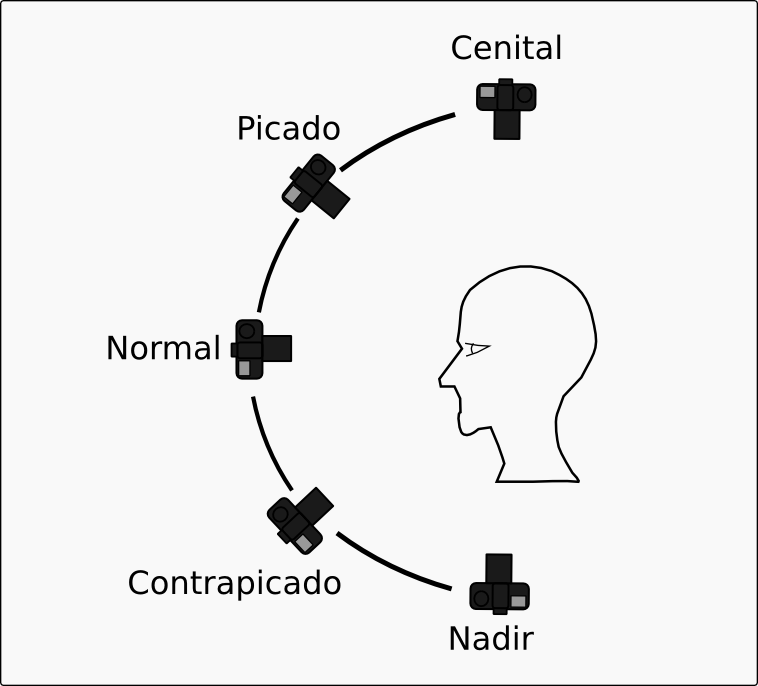
\includegraphics[width=6cm]{otros/manual/angulos.png}}
	\caption{Ángulos posibles}
	\label{mec:angulos}
\end{figure}

\begin{itemize}
	\item \textbf{Juego de lucha uno contra uno o \textit{1v1}}: Implica que dos personajes con exactamente las mismas capacidades, acciones posibles y atributos competirán en el mismo entorno. En lo que a la competición se refiere no existe ninguna entidad más involucrada por lo que el factor decisivo a la hora de determinar un ganador serán las habilidades de quien sea que controle a los personajes.
	\item \textbf{Top-Down}: Vista que en videojuegos se puede referir tanto a un plano cenital\footnote{en fotografía, el punto de vista de la cámara se encuentra perpendicular al suelo} como a un plano picado\footnote{en fotografía, el punto de vista de la cámara tiene un ángulo superior a 45 grados pero sin llegar a 90 con respecto al suelo}, se pueden ver ejemplos en la figura \ref{mec:angulos}. En el presente caso se utiliza un \textbf{plano picado}.
	\item \textbf{En dos dimensiones}: Pues el contenido del videojuego son imágenes planas dibujadas para representar los diferentes estados de los personajes, en ningún momento se utiliza ningún modelo entres dimensiones.
\end{itemize}

\bigskip

En lo referente a las \textbf{mecánicas} presentes en el combate se ha optado por un subconjunto de acciones reducido pero con cierta profundidad. Un personaje puede moverse libremente por la zona de combate que se limita por cuatro paredes (habitación rectangular). Además podrá atacar en la zona justo enfrente de él y defenderse de ataques que vienen desde cualquier dirección. Se explican las interacciones entre mecánicas en las siguientes líneas:

\begin{itemize}
	\item \textbf{Movimiento}: El hecho de moverse libremente en una área limitada hace que se genere naturalmente la necesidad de evitar situaciones en las que no se pueda escapar del contrincante. De forma similar al \textit{control del ring} en boxeo, es necesario tener hacia donde moverse si se requiere por lo que se añade la complejidad de evitar quedar atrapado entre los muros y el enemigo. Además la única forma de cambiar el ángulo hacia el que se está mirando es moverse hacia esa dirección.
	\item \textbf{Ataque}: Al poder atacar simplemente en la zona directamente enfrente del personaje se hace relevante la dirección hacia la que el mismo está mirando. Pese a que pueda parecer baladí esto hace que se beneficie una actitud agresiva al tener que moverte hacia la dirección del enemigo justo antes de atacar para estar mirando en su dirección.
	\item \textbf{Defensa}: Existe la posibilidad de ejecutar un movimiento defensivo que protege del ataque. Es la maniobra que representa un alto riesgo pero una alta recompensa ya que si se consigue defenderse de un ataque se proporciona la posibilidad de realizar un ataque propio sin consecuencias. Por otro lado, si la defensa no recibe ataques se entra en un periodo de descanso o \textit{cooldown} en el que el personaje es vulnerable.
\end{itemize}

\bigskip

La interacción entre movimiento, defensa y ataque crea situaciones en las que no está determinada la mejor estrategia claramente. Un estilo agresivo es castigado por un estilo defensivo, el estilo defensivo pierde ante un jugador pasivo que simplemente espera a que se entre en la fase vulnerable de la defensa y a su vez el jugador pasivo perderá ante uno agresivo. La clásica fórmula de \textit{piedra-papel-tijeras} aplicada de un contexto continuo ha probado ser efectiva en diseño de videojuegos desde el nacimiento de la industria.

\bigskip

Al no favorecer ningún estilo de juego concreto se abren posibilidades sobre que comportamiento es el idóneo para un posible agente complejo. En el siguiente apartado se comenta el algoritmo utilizado para aprender y jugar al videojuego.

\subsection{Algoritmo}

El algoritmo implementado recuerda ligeramente a una versión muy simplificada de \textit{Q-Learning}\footnote{Explicación simple de \textit{Q-Learning} en: \url{http://mnemstudio.org/path-finding-q-learning-tutorial.htm}}. Dada la acción correctiva mostrada en el apartado \ref{AC} se ha optado por una aproximación específica para el problema actual en lugar de realizar implementaciones desde cero de técnicas de aprendizaje por refuerzo. Las mismas requerirían una cantidad de tiempo y recursos del que no se disponía en el proyecto, sin embargo, en el apartado de conclusiones y posibles ampliaciones (\ref{cap:conclusiones}) se especifican las técnicas que sería posible agregar sin demasiado esfuerzo adicional.

\bigskip

El primer paso para hacer funcionar el algoritmo es considerar como discretizar los estados. Existen técnicas relativamente complejas dedicadas a ello como los \textit{mapas auto-organizados}\footnote{tipo de red neuronal artificial entrenado para representar de forma discreta un espacio de entrada de estados continuos}. Se ha optado por una discretización manual en la cual los estados continuos del combate generan una estructura que tiene en cuenta los siguientes datos:

\begin{itemize}
	\item \textbf{Vida de los personajes}: En 5 posibles valores, desde 0 (vacía) hasta 5 (completa).
	\item \textbf{Acción que se está realizando}: Que puede ser moverse, atacar, defender, estar quieto o estar descansando de una defensa.
	\item \textbf{Dirección relativa de los personajes}: Se calcula la dirección del enemigo de forma discreta (hacia arriba, abajo, izquierda o derecha).
	\item \textbf{Distancia entre los personajes}: Que se subdivide en tres estados dependiendo del rango de ataque: fuera de rango, cerca de rango o dentro de rango.
	\item \textbf{Posición de los muros}: Se guarda si hay algún muro al lado del personaje que impida su movimiento.
	\item \textbf{Si se está mirando al enemigo}: Indica si se está mirando en la dirección del enemigo para poder atacarlo.
\end{itemize}

Una vez discretizados los estados se puede proceder a definir como el agente los irá explorando, así como la manera de asociar una recompensa a la mejor acción para cada estado. Para ello se necesita una función de utilidad o \textit{fitness} que se define teniendo en cuenta:

\begin{itemize}
	\item \textbf{Distancia al enemigo}: Se recompensa al personaje cuando se acerca al enemigo para favorecer un comportamiento agresivo.
	\item \textbf{Vida propia del enemigo}: Se recompensa al personaje cuanta más vida tenga y cuanta menos tenga el enemigo.
	\item \textbf{Posición de los muros}: Se recompensa al personaje si no está al lado de ningún muro que impida el movimiento en esa dirección.
	\item \textbf{Si se está mirando al enemigo}: Se recompensa al personaje si está mirando al enemigo ya que esto posibilita realizar un eventual ataque exitoso.
\end{itemize}

\bigskip

Por otra parte, las acciones discretas que puede realizar el jugador son sencillas: Atacar, defenderse, moverse en cuatro direcciones (arriba, abajo, izquierda o derecha) o quedarse quieto.

\bigskip

Ahora que se cuenta con una función de utilidad, estados discretos y acciones discretas se procede a definir como el agente aprende y escoge entre las diferentes opciones en el \textbf{algoritmo} \ref{algoritmo}.

\bigskip


En el mismo se muestra como en cada iteración del bucle que ejecuta el agente primero se guardará la información referente al estado anterior, la acción elegida y la mejora en \textit{fitness} asociada. Después de esto se escogerá o bien una acción aleatoria si no se conoce el estado o una de entre las que mejor \textit{fitness} tendrán con una probabilidad.

\bigskip


\textbf{$\epsilon$} representa una cantidad entre 0 y 1 que indica que porcentaje de las veces que se elige sobre un estado conocido se decide explorar un estado aleatorio en lugar de  elegir uno de los visitados. Se han utilizado valores cercanos a $0.30$ durante el entrenamiento y se han disminuido a valores ligeramente menores a $0.1$ al finalizar el mismo con la intención de comprobar sus habilidades.


\begin{algorithm}
	
	\SetKwData{Action}{action}
	\SetKwData{LastAction}{selectedAction}
	\SetKwData{LastState}{lastState}
	\SetKwData{CurrentState}{currentState}
	\SetKwData{DeltaFitness}{deltaFitness}
	\SetKwData{StateActionData}{stateActionData}
	\SetKwData{RandomAction}{randomAction}
	\SetKwData{AllActions}{allPosibleActions}
	
	\SetKwFunction{GetRandomAction}{getRandomAction}
	\SetKwFunction{GetCurrentState}{getCurrentState}
	\SetKwFunction{RandomBet}{randomBetween}
	\SetKwFunction{CalculateFitness}{calculateFitness}
	\SetKwFunction{UpdateWith}{updateWith}
	\SetKwFunction{Insert}{insert}
	\SetKwFunction{Pick}{bestWeightedAction}

	\While{agent is running}{
		\LastState$\leftarrow$ \CurrentState\;
		\CurrentState$\leftarrow$ \GetCurrentState{}\;

		\DeltaFitness$\leftarrow$ \CalculateFitness{\CurrentState}$-$\CalculateFitness{\LastState}\;
	
		%Actualizamos el conocimiento del agente
		\uIf{\LastState$\in$ \StateActionData}{
			\StateActionData$.$\UpdateWith{\LastState,\LastAction,\DeltaFitness}\;
		}
		\Else{
			\StateActionData$.$\Insert{\LastState,\LastAction,\DeltaFitness}\;
		}
	
	
		%Seleccionamos la acción a escoger
		\uIf{\CurrentState$\in$ \StateActionData}{
			
			\uIf{\RandomBet{$0$,$1$}$<\epsilon$}{
				\LastAction$\leftarrow$ \RandomAction $\in$ \AllActions\;
			}
			\Else{
				\LastAction$\leftarrow$ \Action $\in$ \AllActions  $|$ \Pick{\StateActionData,\CurrentState} $=$ \Action  \;
			}
			
		}
		\Else{
			\LastAction$\leftarrow$ \RandomAction $\in$ \AllActions\;
		}
	
	
	}
	\caption{Algoritmo general del agente}
	\label{algoritmo}
\end{algorithm}

 
